\documentclass[11pt]{article}

    \usepackage[breakable]{tcolorbox}
    \usepackage{parskip} % Stop auto-indenting (to mimic markdown behaviour)
    
    \usepackage{iftex}
    \ifPDFTeX
    	\usepackage[T1]{fontenc}
    	\usepackage{mathpazo}
    \else
    	\usepackage{fontspec}
    \fi

    % Basic figure setup, for now with no caption control since it's done
    % automatically by Pandoc (which extracts ![](path) syntax from Markdown).
    \usepackage{graphicx}
    % Maintain compatibility with old templates. Remove in nbconvert 6.0
    \let\Oldincludegraphics\includegraphics
    % Ensure that by default, figures have no caption (until we provide a
    % proper Figure object with a Caption API and a way to capture that
    % in the conversion process - todo).
    \usepackage{caption}
    \DeclareCaptionFormat{nocaption}{}
    \captionsetup{format=nocaption,aboveskip=0pt,belowskip=0pt}

    \usepackage[Export]{adjustbox} % Used to constrain images to a maximum size
    \adjustboxset{max size={0.9\linewidth}{0.9\paperheight}}
    \usepackage{float}
    \floatplacement{figure}{H} % forces figures to be placed at the correct location
    \usepackage{xcolor} % Allow colors to be defined
    \usepackage{enumerate} % Needed for markdown enumerations to work
    \usepackage{geometry} % Used to adjust the document margins
    \usepackage{amsmath} % Equations
    \usepackage{amssymb} % Equations
    \usepackage{textcomp} % defines textquotesingle
    % Hack from http://tex.stackexchange.com/a/47451/13684:
    \AtBeginDocument{%
        \def\PYZsq{\textquotesingle}% Upright quotes in Pygmentized code
    }
    \usepackage{upquote} % Upright quotes for verbatim code
    \usepackage{eurosym} % defines \euro
    \usepackage[mathletters]{ucs} % Extended unicode (utf-8) support
    \usepackage{fancyvrb} % verbatim replacement that allows latex

    % The hyperref package gives us a pdf with properly built
    % internal navigation ('pdf bookmarks' for the table of contents,
    % internal cross-reference links, web links for URLs, etc.)
    \usepackage{hyperref}
    % The default LaTeX title has an obnoxious amount of whitespace. By default,
    % titling removes some of it. It also provides customization options.
    \usepackage{titling}
    \usepackage{longtable} % longtable support required by pandoc >1.10
    \usepackage{booktabs}  % table support for pandoc > 1.12.2
    \usepackage[inline]{enumitem} % IRkernel/repr support (it uses the enumerate* environment)
    \usepackage[normalem]{ulem} % ulem is needed to support strikethroughs (\sout)
                                % normalem makes italics be italics, not underlines
    \usepackage{mathrsfs}
    

    
    % Colors for the hyperref package
    \definecolor{urlcolor}{rgb}{0,.145,.698}
    \definecolor{linkcolor}{rgb}{.71,0.21,0.01}
    \definecolor{citecolor}{rgb}{.12,.54,.11}

    % ANSI colors
    \definecolor{ansi-black}{HTML}{3E424D}
    \definecolor{ansi-black-intense}{HTML}{282C36}
    \definecolor{ansi-red}{HTML}{E75C58}
    \definecolor{ansi-red-intense}{HTML}{B22B31}
    \definecolor{ansi-green}{HTML}{00A250}
    \definecolor{ansi-green-intense}{HTML}{007427}
    \definecolor{ansi-yellow}{HTML}{DDB62B}
    \definecolor{ansi-yellow-intense}{HTML}{B27D12}
    \definecolor{ansi-blue}{HTML}{208FFB}
    \definecolor{ansi-blue-intense}{HTML}{0065CA}
    \definecolor{ansi-magenta}{HTML}{D160C4}
    \definecolor{ansi-magenta-intense}{HTML}{A03196}
    \definecolor{ansi-cyan}{HTML}{60C6C8}
    \definecolor{ansi-cyan-intense}{HTML}{258F8F}
    \definecolor{ansi-white}{HTML}{C5C1B4}
    \definecolor{ansi-white-intense}{HTML}{A1A6B2}
    \definecolor{ansi-default-inverse-fg}{HTML}{FFFFFF}
    \definecolor{ansi-default-inverse-bg}{HTML}{000000}

    % commands and environments needed by pandoc snippets
    % extracted from the output of `pandoc -s`
    \providecommand{\tightlist}{%
      \setlength{\itemsep}{0pt}\setlength{\parskip}{0pt}}
    \DefineVerbatimEnvironment{Highlighting}{Verbatim}{commandchars=\\\{\}}
    % Add ',fontsize=\small' for more characters per line
    \newenvironment{Shaded}{}{}
    \newcommand{\KeywordTok}[1]{\textcolor[rgb]{0.00,0.44,0.13}{\textbf{{#1}}}}
    \newcommand{\DataTypeTok}[1]{\textcolor[rgb]{0.56,0.13,0.00}{{#1}}}
    \newcommand{\DecValTok}[1]{\textcolor[rgb]{0.25,0.63,0.44}{{#1}}}
    \newcommand{\BaseNTok}[1]{\textcolor[rgb]{0.25,0.63,0.44}{{#1}}}
    \newcommand{\FloatTok}[1]{\textcolor[rgb]{0.25,0.63,0.44}{{#1}}}
    \newcommand{\CharTok}[1]{\textcolor[rgb]{0.25,0.44,0.63}{{#1}}}
    \newcommand{\StringTok}[1]{\textcolor[rgb]{0.25,0.44,0.63}{{#1}}}
    \newcommand{\CommentTok}[1]{\textcolor[rgb]{0.38,0.63,0.69}{\textit{{#1}}}}
    \newcommand{\OtherTok}[1]{\textcolor[rgb]{0.00,0.44,0.13}{{#1}}}
    \newcommand{\AlertTok}[1]{\textcolor[rgb]{1.00,0.00,0.00}{\textbf{{#1}}}}
    \newcommand{\FunctionTok}[1]{\textcolor[rgb]{0.02,0.16,0.49}{{#1}}}
    \newcommand{\RegionMarkerTok}[1]{{#1}}
    \newcommand{\ErrorTok}[1]{\textcolor[rgb]{1.00,0.00,0.00}{\textbf{{#1}}}}
    \newcommand{\NormalTok}[1]{{#1}}
    
    % Additional commands for more recent versions of Pandoc
    \newcommand{\ConstantTok}[1]{\textcolor[rgb]{0.53,0.00,0.00}{{#1}}}
    \newcommand{\SpecialCharTok}[1]{\textcolor[rgb]{0.25,0.44,0.63}{{#1}}}
    \newcommand{\VerbatimStringTok}[1]{\textcolor[rgb]{0.25,0.44,0.63}{{#1}}}
    \newcommand{\SpecialStringTok}[1]{\textcolor[rgb]{0.73,0.40,0.53}{{#1}}}
    \newcommand{\ImportTok}[1]{{#1}}
    \newcommand{\DocumentationTok}[1]{\textcolor[rgb]{0.73,0.13,0.13}{\textit{{#1}}}}
    \newcommand{\AnnotationTok}[1]{\textcolor[rgb]{0.38,0.63,0.69}{\textbf{\textit{{#1}}}}}
    \newcommand{\CommentVarTok}[1]{\textcolor[rgb]{0.38,0.63,0.69}{\textbf{\textit{{#1}}}}}
    \newcommand{\VariableTok}[1]{\textcolor[rgb]{0.10,0.09,0.49}{{#1}}}
    \newcommand{\ControlFlowTok}[1]{\textcolor[rgb]{0.00,0.44,0.13}{\textbf{{#1}}}}
    \newcommand{\OperatorTok}[1]{\textcolor[rgb]{0.40,0.40,0.40}{{#1}}}
    \newcommand{\BuiltInTok}[1]{{#1}}
    \newcommand{\ExtensionTok}[1]{{#1}}
    \newcommand{\PreprocessorTok}[1]{\textcolor[rgb]{0.74,0.48,0.00}{{#1}}}
    \newcommand{\AttributeTok}[1]{\textcolor[rgb]{0.49,0.56,0.16}{{#1}}}
    \newcommand{\InformationTok}[1]{\textcolor[rgb]{0.38,0.63,0.69}{\textbf{\textit{{#1}}}}}
    \newcommand{\WarningTok}[1]{\textcolor[rgb]{0.38,0.63,0.69}{\textbf{\textit{{#1}}}}}
    
    
    % Define a nice break command that doesn't care if a line doesn't already
    % exist.
    \def\br{\hspace*{\fill} \\* }
    % Math Jax compatibility definitions
    \def\gt{>}
    \def\lt{<}
    \let\Oldtex\TeX
    \let\Oldlatex\LaTeX
    \renewcommand{\TeX}{\textrm{\Oldtex}}
    \renewcommand{\LaTeX}{\textrm{\Oldlatex}}
    % Document parameters
    % Document title
    \title{%
    CSE 401: Artificial Intelligence \\
    \Large Tic-Tac-Toe Game using MiniMax Algorithm}

    \author{%
      Utkarsh Gupta \\
      \small A2305217557 \\
      \small 7CSE 8Y}
    \date{August 25th, 2020}
    
    
    
    
% Pygments definitions
\makeatletter
\def\PY@reset{\let\PY@it=\relax \let\PY@bf=\relax%
    \let\PY@ul=\relax \let\PY@tc=\relax%
    \let\PY@bc=\relax \let\PY@ff=\relax}
\def\PY@tok#1{\csname PY@tok@#1\endcsname}
\def\PY@toks#1+{\ifx\relax#1\empty\else%
    \PY@tok{#1}\expandafter\PY@toks\fi}
\def\PY@do#1{\PY@bc{\PY@tc{\PY@ul{%
    \PY@it{\PY@bf{\PY@ff{#1}}}}}}}
\def\PY#1#2{\PY@reset\PY@toks#1+\relax+\PY@do{#2}}

\expandafter\def\csname PY@tok@w\endcsname{\def\PY@tc##1{\textcolor[rgb]{0.73,0.73,0.73}{##1}}}
\expandafter\def\csname PY@tok@c\endcsname{\let\PY@it=\textit\def\PY@tc##1{\textcolor[rgb]{0.25,0.50,0.50}{##1}}}
\expandafter\def\csname PY@tok@cp\endcsname{\def\PY@tc##1{\textcolor[rgb]{0.74,0.48,0.00}{##1}}}
\expandafter\def\csname PY@tok@k\endcsname{\let\PY@bf=\textbf\def\PY@tc##1{\textcolor[rgb]{0.00,0.50,0.00}{##1}}}
\expandafter\def\csname PY@tok@kp\endcsname{\def\PY@tc##1{\textcolor[rgb]{0.00,0.50,0.00}{##1}}}
\expandafter\def\csname PY@tok@kt\endcsname{\def\PY@tc##1{\textcolor[rgb]{0.69,0.00,0.25}{##1}}}
\expandafter\def\csname PY@tok@o\endcsname{\def\PY@tc##1{\textcolor[rgb]{0.40,0.40,0.40}{##1}}}
\expandafter\def\csname PY@tok@ow\endcsname{\let\PY@bf=\textbf\def\PY@tc##1{\textcolor[rgb]{0.67,0.13,1.00}{##1}}}
\expandafter\def\csname PY@tok@nb\endcsname{\def\PY@tc##1{\textcolor[rgb]{0.00,0.50,0.00}{##1}}}
\expandafter\def\csname PY@tok@nf\endcsname{\def\PY@tc##1{\textcolor[rgb]{0.00,0.00,1.00}{##1}}}
\expandafter\def\csname PY@tok@nc\endcsname{\let\PY@bf=\textbf\def\PY@tc##1{\textcolor[rgb]{0.00,0.00,1.00}{##1}}}
\expandafter\def\csname PY@tok@nn\endcsname{\let\PY@bf=\textbf\def\PY@tc##1{\textcolor[rgb]{0.00,0.00,1.00}{##1}}}
\expandafter\def\csname PY@tok@ne\endcsname{\let\PY@bf=\textbf\def\PY@tc##1{\textcolor[rgb]{0.82,0.25,0.23}{##1}}}
\expandafter\def\csname PY@tok@nv\endcsname{\def\PY@tc##1{\textcolor[rgb]{0.10,0.09,0.49}{##1}}}
\expandafter\def\csname PY@tok@no\endcsname{\def\PY@tc##1{\textcolor[rgb]{0.53,0.00,0.00}{##1}}}
\expandafter\def\csname PY@tok@nl\endcsname{\def\PY@tc##1{\textcolor[rgb]{0.63,0.63,0.00}{##1}}}
\expandafter\def\csname PY@tok@ni\endcsname{\let\PY@bf=\textbf\def\PY@tc##1{\textcolor[rgb]{0.60,0.60,0.60}{##1}}}
\expandafter\def\csname PY@tok@na\endcsname{\def\PY@tc##1{\textcolor[rgb]{0.49,0.56,0.16}{##1}}}
\expandafter\def\csname PY@tok@nt\endcsname{\let\PY@bf=\textbf\def\PY@tc##1{\textcolor[rgb]{0.00,0.50,0.00}{##1}}}
\expandafter\def\csname PY@tok@nd\endcsname{\def\PY@tc##1{\textcolor[rgb]{0.67,0.13,1.00}{##1}}}
\expandafter\def\csname PY@tok@s\endcsname{\def\PY@tc##1{\textcolor[rgb]{0.73,0.13,0.13}{##1}}}
\expandafter\def\csname PY@tok@sd\endcsname{\let\PY@it=\textit\def\PY@tc##1{\textcolor[rgb]{0.73,0.13,0.13}{##1}}}
\expandafter\def\csname PY@tok@si\endcsname{\let\PY@bf=\textbf\def\PY@tc##1{\textcolor[rgb]{0.73,0.40,0.53}{##1}}}
\expandafter\def\csname PY@tok@se\endcsname{\let\PY@bf=\textbf\def\PY@tc##1{\textcolor[rgb]{0.73,0.40,0.13}{##1}}}
\expandafter\def\csname PY@tok@sr\endcsname{\def\PY@tc##1{\textcolor[rgb]{0.73,0.40,0.53}{##1}}}
\expandafter\def\csname PY@tok@ss\endcsname{\def\PY@tc##1{\textcolor[rgb]{0.10,0.09,0.49}{##1}}}
\expandafter\def\csname PY@tok@sx\endcsname{\def\PY@tc##1{\textcolor[rgb]{0.00,0.50,0.00}{##1}}}
\expandafter\def\csname PY@tok@m\endcsname{\def\PY@tc##1{\textcolor[rgb]{0.40,0.40,0.40}{##1}}}
\expandafter\def\csname PY@tok@gh\endcsname{\let\PY@bf=\textbf\def\PY@tc##1{\textcolor[rgb]{0.00,0.00,0.50}{##1}}}
\expandafter\def\csname PY@tok@gu\endcsname{\let\PY@bf=\textbf\def\PY@tc##1{\textcolor[rgb]{0.50,0.00,0.50}{##1}}}
\expandafter\def\csname PY@tok@gd\endcsname{\def\PY@tc##1{\textcolor[rgb]{0.63,0.00,0.00}{##1}}}
\expandafter\def\csname PY@tok@gi\endcsname{\def\PY@tc##1{\textcolor[rgb]{0.00,0.63,0.00}{##1}}}
\expandafter\def\csname PY@tok@gr\endcsname{\def\PY@tc##1{\textcolor[rgb]{1.00,0.00,0.00}{##1}}}
\expandafter\def\csname PY@tok@ge\endcsname{\let\PY@it=\textit}
\expandafter\def\csname PY@tok@gs\endcsname{\let\PY@bf=\textbf}
\expandafter\def\csname PY@tok@gp\endcsname{\let\PY@bf=\textbf\def\PY@tc##1{\textcolor[rgb]{0.00,0.00,0.50}{##1}}}
\expandafter\def\csname PY@tok@go\endcsname{\def\PY@tc##1{\textcolor[rgb]{0.53,0.53,0.53}{##1}}}
\expandafter\def\csname PY@tok@gt\endcsname{\def\PY@tc##1{\textcolor[rgb]{0.00,0.27,0.87}{##1}}}
\expandafter\def\csname PY@tok@err\endcsname{\def\PY@bc##1{\setlength{\fboxsep}{0pt}\fcolorbox[rgb]{1.00,0.00,0.00}{1,1,1}{\strut ##1}}}
\expandafter\def\csname PY@tok@kc\endcsname{\let\PY@bf=\textbf\def\PY@tc##1{\textcolor[rgb]{0.00,0.50,0.00}{##1}}}
\expandafter\def\csname PY@tok@kd\endcsname{\let\PY@bf=\textbf\def\PY@tc##1{\textcolor[rgb]{0.00,0.50,0.00}{##1}}}
\expandafter\def\csname PY@tok@kn\endcsname{\let\PY@bf=\textbf\def\PY@tc##1{\textcolor[rgb]{0.00,0.50,0.00}{##1}}}
\expandafter\def\csname PY@tok@kr\endcsname{\let\PY@bf=\textbf\def\PY@tc##1{\textcolor[rgb]{0.00,0.50,0.00}{##1}}}
\expandafter\def\csname PY@tok@bp\endcsname{\def\PY@tc##1{\textcolor[rgb]{0.00,0.50,0.00}{##1}}}
\expandafter\def\csname PY@tok@fm\endcsname{\def\PY@tc##1{\textcolor[rgb]{0.00,0.00,1.00}{##1}}}
\expandafter\def\csname PY@tok@vc\endcsname{\def\PY@tc##1{\textcolor[rgb]{0.10,0.09,0.49}{##1}}}
\expandafter\def\csname PY@tok@vg\endcsname{\def\PY@tc##1{\textcolor[rgb]{0.10,0.09,0.49}{##1}}}
\expandafter\def\csname PY@tok@vi\endcsname{\def\PY@tc##1{\textcolor[rgb]{0.10,0.09,0.49}{##1}}}
\expandafter\def\csname PY@tok@vm\endcsname{\def\PY@tc##1{\textcolor[rgb]{0.10,0.09,0.49}{##1}}}
\expandafter\def\csname PY@tok@sa\endcsname{\def\PY@tc##1{\textcolor[rgb]{0.73,0.13,0.13}{##1}}}
\expandafter\def\csname PY@tok@sb\endcsname{\def\PY@tc##1{\textcolor[rgb]{0.73,0.13,0.13}{##1}}}
\expandafter\def\csname PY@tok@sc\endcsname{\def\PY@tc##1{\textcolor[rgb]{0.73,0.13,0.13}{##1}}}
\expandafter\def\csname PY@tok@dl\endcsname{\def\PY@tc##1{\textcolor[rgb]{0.73,0.13,0.13}{##1}}}
\expandafter\def\csname PY@tok@s2\endcsname{\def\PY@tc##1{\textcolor[rgb]{0.73,0.13,0.13}{##1}}}
\expandafter\def\csname PY@tok@sh\endcsname{\def\PY@tc##1{\textcolor[rgb]{0.73,0.13,0.13}{##1}}}
\expandafter\def\csname PY@tok@s1\endcsname{\def\PY@tc##1{\textcolor[rgb]{0.73,0.13,0.13}{##1}}}
\expandafter\def\csname PY@tok@mb\endcsname{\def\PY@tc##1{\textcolor[rgb]{0.40,0.40,0.40}{##1}}}
\expandafter\def\csname PY@tok@mf\endcsname{\def\PY@tc##1{\textcolor[rgb]{0.40,0.40,0.40}{##1}}}
\expandafter\def\csname PY@tok@mh\endcsname{\def\PY@tc##1{\textcolor[rgb]{0.40,0.40,0.40}{##1}}}
\expandafter\def\csname PY@tok@mi\endcsname{\def\PY@tc##1{\textcolor[rgb]{0.40,0.40,0.40}{##1}}}
\expandafter\def\csname PY@tok@il\endcsname{\def\PY@tc##1{\textcolor[rgb]{0.40,0.40,0.40}{##1}}}
\expandafter\def\csname PY@tok@mo\endcsname{\def\PY@tc##1{\textcolor[rgb]{0.40,0.40,0.40}{##1}}}
\expandafter\def\csname PY@tok@ch\endcsname{\let\PY@it=\textit\def\PY@tc##1{\textcolor[rgb]{0.25,0.50,0.50}{##1}}}
\expandafter\def\csname PY@tok@cm\endcsname{\let\PY@it=\textit\def\PY@tc##1{\textcolor[rgb]{0.25,0.50,0.50}{##1}}}
\expandafter\def\csname PY@tok@cpf\endcsname{\let\PY@it=\textit\def\PY@tc##1{\textcolor[rgb]{0.25,0.50,0.50}{##1}}}
\expandafter\def\csname PY@tok@c1\endcsname{\let\PY@it=\textit\def\PY@tc##1{\textcolor[rgb]{0.25,0.50,0.50}{##1}}}
\expandafter\def\csname PY@tok@cs\endcsname{\let\PY@it=\textit\def\PY@tc##1{\textcolor[rgb]{0.25,0.50,0.50}{##1}}}

\def\PYZbs{\char`\\}
\def\PYZus{\char`\_}
\def\PYZob{\char`\{}
\def\PYZcb{\char`\}}
\def\PYZca{\char`\^}
\def\PYZam{\char`\&}
\def\PYZlt{\char`\<}
\def\PYZgt{\char`\>}
\def\PYZsh{\char`\#}
\def\PYZpc{\char`\%}
\def\PYZdl{\char`\$}
\def\PYZhy{\char`\-}
\def\PYZsq{\char`\'}
\def\PYZdq{\char`\"}
\def\PYZti{\char`\~}
% for compatibility with earlier versions
\def\PYZat{@}
\def\PYZlb{[}
\def\PYZrb{]}
\makeatother


    % For linebreaks inside Verbatim environment from package fancyvrb. 
    \makeatletter
        \newbox\Wrappedcontinuationbox 
        \newbox\Wrappedvisiblespacebox 
        \newcommand*\Wrappedvisiblespace {\textcolor{red}{\textvisiblespace}} 
        \newcommand*\Wrappedcontinuationsymbol {\textcolor{red}{\llap{\tiny$\m@th\hookrightarrow$}}} 
        \newcommand*\Wrappedcontinuationindent {3ex } 
        \newcommand*\Wrappedafterbreak {\kern\Wrappedcontinuationindent\copy\Wrappedcontinuationbox} 
        % Take advantage of the already applied Pygments mark-up to insert 
        % potential linebreaks for TeX processing. 
        %        {, <, #, %, $, ' and ": go to next line. 
        %        _, }, ^, &, >, - and ~: stay at end of broken line. 
        % Use of \textquotesingle for straight quote. 
        \newcommand*\Wrappedbreaksatspecials {% 
            \def\PYGZus{\discretionary{\char`\_}{\Wrappedafterbreak}{\char`\_}}% 
            \def\PYGZob{\discretionary{}{\Wrappedafterbreak\char`\{}{\char`\{}}% 
            \def\PYGZcb{\discretionary{\char`\}}{\Wrappedafterbreak}{\char`\}}}% 
            \def\PYGZca{\discretionary{\char`\^}{\Wrappedafterbreak}{\char`\^}}% 
            \def\PYGZam{\discretionary{\char`\&}{\Wrappedafterbreak}{\char`\&}}% 
            \def\PYGZlt{\discretionary{}{\Wrappedafterbreak\char`\<}{\char`\<}}% 
            \def\PYGZgt{\discretionary{\char`\>}{\Wrappedafterbreak}{\char`\>}}% 
            \def\PYGZsh{\discretionary{}{\Wrappedafterbreak\char`\#}{\char`\#}}% 
            \def\PYGZpc{\discretionary{}{\Wrappedafterbreak\char`\%}{\char`\%}}% 
            \def\PYGZdl{\discretionary{}{\Wrappedafterbreak\char`\$}{\char`\$}}% 
            \def\PYGZhy{\discretionary{\char`\-}{\Wrappedafterbreak}{\char`\-}}% 
            \def\PYGZsq{\discretionary{}{\Wrappedafterbreak\textquotesingle}{\textquotesingle}}% 
            \def\PYGZdq{\discretionary{}{\Wrappedafterbreak\char`\"}{\char`\"}}% 
            \def\PYGZti{\discretionary{\char`\~}{\Wrappedafterbreak}{\char`\~}}% 
        } 
        % Some characters . , ; ? ! / are not pygmentized. 
        % This macro makes them "active" and they will insert potential linebreaks 
        \newcommand*\Wrappedbreaksatpunct {% 
            \lccode`\~`\.\lowercase{\def~}{\discretionary{\hbox{\char`\.}}{\Wrappedafterbreak}{\hbox{\char`\.}}}% 
            \lccode`\~`\,\lowercase{\def~}{\discretionary{\hbox{\char`\,}}{\Wrappedafterbreak}{\hbox{\char`\,}}}% 
            \lccode`\~`\;\lowercase{\def~}{\discretionary{\hbox{\char`\;}}{\Wrappedafterbreak}{\hbox{\char`\;}}}% 
            \lccode`\~`\:\lowercase{\def~}{\discretionary{\hbox{\char`\:}}{\Wrappedafterbreak}{\hbox{\char`\:}}}% 
            \lccode`\~`\?\lowercase{\def~}{\discretionary{\hbox{\char`\?}}{\Wrappedafterbreak}{\hbox{\char`\?}}}% 
            \lccode`\~`\!\lowercase{\def~}{\discretionary{\hbox{\char`\!}}{\Wrappedafterbreak}{\hbox{\char`\!}}}% 
            \lccode`\~`\/\lowercase{\def~}{\discretionary{\hbox{\char`\/}}{\Wrappedafterbreak}{\hbox{\char`\/}}}% 
            \catcode`\.\active
            \catcode`\,\active 
            \catcode`\;\active
            \catcode`\:\active
            \catcode`\?\active
            \catcode`\!\active
            \catcode`\/\active 
            \lccode`\~`\~ 	
        }
    \makeatother

    \let\OriginalVerbatim=\Verbatim
    \makeatletter
    \renewcommand{\Verbatim}[1][1]{%
        %\parskip\z@skip
        \sbox\Wrappedcontinuationbox {\Wrappedcontinuationsymbol}%
        \sbox\Wrappedvisiblespacebox {\FV@SetupFont\Wrappedvisiblespace}%
        \def\FancyVerbFormatLine ##1{\hsize\linewidth
            \vtop{\raggedright\hyphenpenalty\z@\exhyphenpenalty\z@
                \doublehyphendemerits\z@\finalhyphendemerits\z@
                \strut ##1\strut}%
        }%
        % If the linebreak is at a space, the latter will be displayed as visible
        % space at end of first line, and a continuation symbol starts next line.
        % Stretch/shrink are however usually zero for typewriter font.
        \def\FV@Space {%
            \nobreak\hskip\z@ plus\fontdimen3\font minus\fontdimen4\font
            \discretionary{\copy\Wrappedvisiblespacebox}{\Wrappedafterbreak}
            {\kern\fontdimen2\font}%
        }%
        
        % Allow breaks at special characters using \PYG... macros.
        \Wrappedbreaksatspecials
        % Breaks at punctuation characters . , ; ? ! and / need catcode=\active 	
        \OriginalVerbatim[#1,codes*=\Wrappedbreaksatpunct]%
    }
    \makeatother

    % Exact colors from NB
    \definecolor{incolor}{HTML}{303F9F}
    \definecolor{outcolor}{HTML}{D84315}
    \definecolor{cellborder}{HTML}{CFCFCF}
    \definecolor{cellbackground}{HTML}{F7F7F7}
    
    % prompt
    \makeatletter
    \newcommand{\boxspacing}{\kern\kvtcb@left@rule\kern\kvtcb@boxsep}
    \makeatother
    \newcommand{\prompt}[4]{
        \ttfamily\llap{{\color{#2}[#3]:\hspace{3pt}#4}}\vspace{-\baselineskip}
    }
    

    
    % Prevent overflowing lines due to hard-to-break entities
    \sloppy 
    % Setup hyperref package
    \hypersetup{
      breaklinks=true,  % so long urls are correctly broken across lines
      colorlinks=true,
      urlcolor=urlcolor,
      linkcolor=linkcolor,
      citecolor=citecolor,
      }
    % Slightly bigger margins than the latex defaults
    
    \geometry{verbose,tmargin=1in,bmargin=1in,lmargin=1in,rmargin=1in}
    
    

\begin{document}
    
    \maketitle
    
    \hypertarget{introduction}{%
\section{What is MiniMax?}\label{introduction}}

Minimax is a artifical intelligence applied in two player games, such as
tic-tac-toe, checkers, chess and go. This games are known as zero-sum
games, because in a mathematical representation: one player wins (+1)
and other player loses (-1) or both of anyone not to win (0).

Minimax is a type of adversarial search algorithm for generating and
exploring game trees. It is mostly used to solve zero-sum games where
one side's gain is equivalent to other side's loss, so adding all gains
and subtracting all losses end up being zero.

Adversarial search differs from conventional searching algorithms by
adding opponents into the mix. Minimax algorithm keeps playing the turns
of both player and the opponent optimally to figure out the best
possible move.

\begin{figure}
\centering
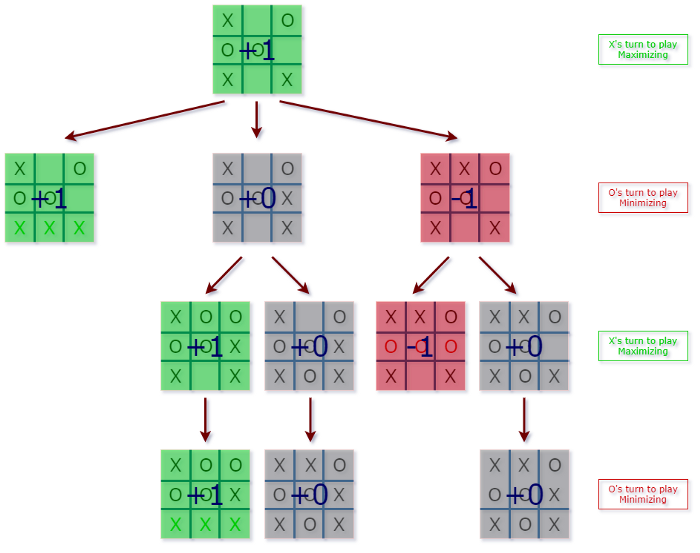
\includegraphics[width=13cm]{assets/minimax.png}
\caption{MiniMax}
\end{figure}

    \hypertarget{how-does-it-work}{%
\section{How does it work?}\label{how-does-it-work}}

The algorithm search, recursively, the best move that leads the Max
player to win or not lose (draw). It consider the current state of the
game and the available moves at that state, then for each valid move it
plays (alternating min and max) until it finds a terminal state (win,
draw or lose).

Minimax is a kind of backtracking algorithm that is used in decision
making and game theory to find the optimal move for a player, assuming
that your opponent also plays optimally. It is widely used in two player
turn-based games such as Tic-Tac-Toe, Backgammon, Mancala, Chess, etc.

In Minimax the two players are called maximizer and minimizer. The
maximizer tries to get the highest score possible while the minimizer
tries to do the opposite and get the lowest score possible.

Every board state has a value associated with it. In a given state if
the maximizer has upper hand then, the score of the board will tend to
be some positive value. If the minimizer has the upper hand in that
board state then it will tend to be some negative value. The values of
the board are calculated by some heuristics which are unique for every
type of game.

Example: Consider a game which has 4 final states and paths to reach
final state are from root to 4 leaves of a perfect binary tree as shown
below. Assume you are the maximizing player and you get the first chance
to move, i.e., you are at the root and your opponent at next level.
Which move you would make as a maximizing player considering that your
opponent also plays optimally?

\begin{figure}
\centering
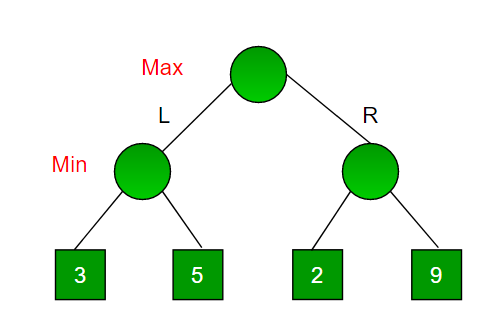
\includegraphics[width=10cm]{assets/example1.png}
\caption{MiniMax}
\end{figure}

Since this is a backtracking based algorithm, it tries all possible
moves, then backtracks and makes a decision.

Maximizer goes LEFT: It is now the minimizers turn. The minimizer now
has a choice between 3 and 5. Being the minimizer it will definitely
choose the least among both, that is 3 Maximizer goes RIGHT: It is now
the minimizers turn. The minimizer now has a choice between 2 and 9. He
will choose 2 as it is the least among the two values. Being the
maximizer you would choose the larger value that is 3. Hence the optimal
move for the maximizer is to go LEFT and the optimal value is 3.

\newpage

Now the game tree looks like below :

\begin{figure}
\centering
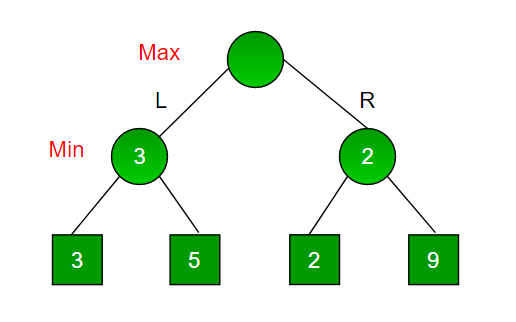
\includegraphics[width=13cm]{assets/example2.png}
\caption{MiniMax}
\end{figure}

The above tree shows two possible scores when maximizer makes left and
right moves.

Note: Even though there is a value of 9 on the right subtree, the
minimizer will never pick that. We must always assume that our opponent
plays optimally.

    ~\\
    \noindent\rule{16.5cm}{0.4pt}
    \newpage
    
    \section{Code}

    \begin{tcolorbox}[breakable, size=fbox, boxrule=1pt, pad at break*=1mm,colback=cellbackground, colframe=cellborder]
\prompt{In}{incolor}{1}{\boxspacing}
\begin{Verbatim}[commandchars=\\\{\}]
\PY{c+c1}{\PYZsh{}Import the necessary libraries}
\PY{k+kn}{import} \PY{n+nn}{numpy} \PY{k}{as} \PY{n+nn}{np}
\PY{k+kn}{from} \PY{n+nn}{math} \PY{k}{import} \PY{n}{inf} \PY{k}{as} \PY{n}{infinity}
\end{Verbatim}
\end{tcolorbox}

    \begin{tcolorbox}[breakable, size=fbox, boxrule=1pt, pad at break*=1mm,colback=cellbackground, colframe=cellborder]
\prompt{In}{incolor}{2}{\boxspacing}
\begin{Verbatim}[commandchars=\\\{\}]
\PY{c+c1}{\PYZsh{}Set the Empty Board}
\PY{n}{game\PYZus{}state} \PY{o}{=} \PY{p}{[}\PY{p}{[}\PY{l+s+s1}{\PYZsq{}}\PY{l+s+s1}{ }\PY{l+s+s1}{\PYZsq{}}\PY{p}{,}\PY{l+s+s1}{\PYZsq{}}\PY{l+s+s1}{ }\PY{l+s+s1}{\PYZsq{}}\PY{p}{,}\PY{l+s+s1}{\PYZsq{}}\PY{l+s+s1}{ }\PY{l+s+s1}{\PYZsq{}}\PY{p}{]}\PY{p}{,}
              \PY{p}{[}\PY{l+s+s1}{\PYZsq{}}\PY{l+s+s1}{ }\PY{l+s+s1}{\PYZsq{}}\PY{p}{,}\PY{l+s+s1}{\PYZsq{}}\PY{l+s+s1}{ }\PY{l+s+s1}{\PYZsq{}}\PY{p}{,}\PY{l+s+s1}{\PYZsq{}}\PY{l+s+s1}{ }\PY{l+s+s1}{\PYZsq{}}\PY{p}{]}\PY{p}{,}
              \PY{p}{[}\PY{l+s+s1}{\PYZsq{}}\PY{l+s+s1}{ }\PY{l+s+s1}{\PYZsq{}}\PY{p}{,}\PY{l+s+s1}{\PYZsq{}}\PY{l+s+s1}{ }\PY{l+s+s1}{\PYZsq{}}\PY{p}{,}\PY{l+s+s1}{\PYZsq{}}\PY{l+s+s1}{ }\PY{l+s+s1}{\PYZsq{}}\PY{p}{]}\PY{p}{]}
\PY{c+c1}{\PYZsh{}Create the Two Players as \PYZsq{}X\PYZsq{}/\PYZsq{}O\PYZsq{}}
\PY{n}{players} \PY{o}{=} \PY{p}{[}\PY{l+s+s1}{\PYZsq{}}\PY{l+s+s1}{X}\PY{l+s+s1}{\PYZsq{}}\PY{p}{,}\PY{l+s+s1}{\PYZsq{}}\PY{l+s+s1}{O}\PY{l+s+s1}{\PYZsq{}}\PY{p}{]}
\end{Verbatim}
\end{tcolorbox}

    \begin{tcolorbox}[breakable, size=fbox, boxrule=1pt, pad at break*=1mm,colback=cellbackground, colframe=cellborder]
\prompt{In}{incolor}{3}{\boxspacing}
\begin{Verbatim}[commandchars=\\\{\}]
\PY{c+c1}{\PYZsh{}Method for checking the correct move on Tic\PYZhy{}Tac\PYZhy{}Toe}
\PY{k}{def} \PY{n+nf}{play\PYZus{}move}\PY{p}{(}\PY{n}{state}\PY{p}{,} \PY{n}{player}\PY{p}{,} \PY{n}{block\PYZus{}num}\PY{p}{)}\PY{p}{:}
    \PY{k}{if} \PY{n}{state}\PY{p}{[}\PY{n+nb}{int}\PY{p}{(}\PY{p}{(}\PY{n}{block\PYZus{}num}\PY{o}{\PYZhy{}}\PY{l+m+mi}{1}\PY{p}{)}\PY{o}{/}\PY{l+m+mi}{3}\PY{p}{)}\PY{p}{]}\PY{p}{[}\PY{p}{(}\PY{n}{block\PYZus{}num}\PY{o}{\PYZhy{}}\PY{l+m+mi}{1}\PY{p}{)}\PY{o}{\PYZpc{}}\PY{k}{3}] == \PYZsq{} \PYZsq{}:
        \PY{n}{state}\PY{p}{[}\PY{n+nb}{int}\PY{p}{(}\PY{p}{(}\PY{n}{block\PYZus{}num}\PY{o}{\PYZhy{}}\PY{l+m+mi}{1}\PY{p}{)}\PY{o}{/}\PY{l+m+mi}{3}\PY{p}{)}\PY{p}{]}\PY{p}{[}\PY{p}{(}\PY{n}{block\PYZus{}num}\PY{o}{\PYZhy{}}\PY{l+m+mi}{1}\PY{p}{)}\PY{o}{\PYZpc{}}\PY{k}{3}] = player
    \PY{k}{else}\PY{p}{:}
        \PY{n}{block\PYZus{}num} \PY{o}{=} \PY{n+nb}{int}\PY{p}{(}\PY{n+nb}{input}\PY{p}{(}\PY{l+s+s2}{\PYZdq{}}\PY{l+s+s2}{Block is not empty, ya blockhead! Choose again: }\PY{l+s+s2}{\PYZdq{}}\PY{p}{)}\PY{p}{)}
        \PY{n}{play\PYZus{}move}\PY{p}{(}\PY{n}{state}\PY{p}{,} \PY{n}{player}\PY{p}{,} \PY{n}{block\PYZus{}num}\PY{p}{)}
        \PY{k+kc}{None}
\end{Verbatim}
\end{tcolorbox}

    \begin{tcolorbox}[breakable, size=fbox, boxrule=1pt, pad at break*=1mm,colback=cellbackground, colframe=cellborder]
\prompt{In}{incolor}{4}{\boxspacing}
\begin{Verbatim}[commandchars=\\\{\}]
\PY{c+c1}{\PYZsh{}Method to copy the current game state to new\PYZus{}state of Tic\PYZhy{}Tac\PYZhy{}Toe}
\PY{k}{def} \PY{n+nf}{copy\PYZus{}game\PYZus{}state}\PY{p}{(}\PY{n}{state}\PY{p}{)}\PY{p}{:}
    \PY{n}{new\PYZus{}state} \PY{o}{=} \PY{p}{[}\PY{p}{[}\PY{l+s+s1}{\PYZsq{}}\PY{l+s+s1}{ }\PY{l+s+s1}{\PYZsq{}}\PY{p}{,}\PY{l+s+s1}{\PYZsq{}}\PY{l+s+s1}{ }\PY{l+s+s1}{\PYZsq{}}\PY{p}{,}\PY{l+s+s1}{\PYZsq{}}\PY{l+s+s1}{ }\PY{l+s+s1}{\PYZsq{}}\PY{p}{]}\PY{p}{,}\PY{p}{[}\PY{l+s+s1}{\PYZsq{}}\PY{l+s+s1}{ }\PY{l+s+s1}{\PYZsq{}}\PY{p}{,}\PY{l+s+s1}{\PYZsq{}}\PY{l+s+s1}{ }\PY{l+s+s1}{\PYZsq{}}\PY{p}{,}\PY{l+s+s1}{\PYZsq{}}\PY{l+s+s1}{ }\PY{l+s+s1}{\PYZsq{}}\PY{p}{]}\PY{p}{,}\PY{p}{[}\PY{l+s+s1}{\PYZsq{}}\PY{l+s+s1}{ }\PY{l+s+s1}{\PYZsq{}}\PY{p}{,}\PY{l+s+s1}{\PYZsq{}}\PY{l+s+s1}{ }\PY{l+s+s1}{\PYZsq{}}\PY{p}{,}\PY{l+s+s1}{\PYZsq{}}\PY{l+s+s1}{ }\PY{l+s+s1}{\PYZsq{}}\PY{p}{]}\PY{p}{]}
    \PY{k}{for} \PY{n}{i} \PY{o+ow}{in} \PY{n+nb}{range}\PY{p}{(}\PY{l+m+mi}{3}\PY{p}{)}\PY{p}{:}
        \PY{k}{for} \PY{n}{j} \PY{o+ow}{in} \PY{n+nb}{range}\PY{p}{(}\PY{l+m+mi}{3}\PY{p}{)}\PY{p}{:}
            \PY{n}{new\PYZus{}state}\PY{p}{[}\PY{n}{i}\PY{p}{]}\PY{p}{[}\PY{n}{j}\PY{p}{]} \PY{o}{=} \PY{n}{state}\PY{p}{[}\PY{n}{i}\PY{p}{]}\PY{p}{[}\PY{n}{j}\PY{p}{]}
    \PY{k}{return} \PY{n}{new\PYZus{}state}
\end{Verbatim}
\end{tcolorbox}

    \begin{tcolorbox}[breakable, size=fbox, boxrule=1pt, pad at break*=1mm,colback=cellbackground, colframe=cellborder]
\prompt{In}{incolor}{5}{\boxspacing}
\begin{Verbatim}[commandchars=\\\{\}]
\PY{c+c1}{\PYZsh{}Method to check the current state of the Tic\PYZhy{}Tac\PYZhy{}Toe}
\PY{k}{def} \PY{n+nf}{check\PYZus{}current\PYZus{}state}\PY{p}{(}\PY{n}{game\PYZus{}state}\PY{p}{)}\PY{p}{:}
    \PY{n}{draw\PYZus{}flag} \PY{o}{=} \PY{l+m+mi}{0}
    \PY{k}{for} \PY{n}{i} \PY{o+ow}{in} \PY{n+nb}{range}\PY{p}{(}\PY{l+m+mi}{3}\PY{p}{)}\PY{p}{:}
        \PY{k}{for} \PY{n}{j} \PY{o+ow}{in} \PY{n+nb}{range}\PY{p}{(}\PY{l+m+mi}{3}\PY{p}{)}\PY{p}{:}
            \PY{k}{if} \PY{n}{game\PYZus{}state}\PY{p}{[}\PY{n}{i}\PY{p}{]}\PY{p}{[}\PY{n}{j}\PY{p}{]} \PY{o}{==} \PY{l+s+s1}{\PYZsq{}}\PY{l+s+s1}{ }\PY{l+s+s1}{\PYZsq{}}\PY{p}{:}
                \PY{n}{draw\PYZus{}flag} \PY{o}{=} \PY{l+m+mi}{1}
    
    \PY{k}{if} \PY{n}{draw\PYZus{}flag} \PY{o}{==} \PY{l+m+mi}{0}\PY{p}{:}
        \PY{k}{return} \PY{k+kc}{None}\PY{p}{,} \PY{l+s+s2}{\PYZdq{}}\PY{l+s+s2}{Draw}\PY{l+s+s2}{\PYZdq{}}
    
    \PY{c+c1}{\PYZsh{} Check horizontals in first row}
    \PY{k}{if} \PY{p}{(}\PY{n}{game\PYZus{}state}\PY{p}{[}\PY{l+m+mi}{0}\PY{p}{]}\PY{p}{[}\PY{l+m+mi}{0}\PY{p}{]} \PY{o}{==} \PY{n}{game\PYZus{}state}\PY{p}{[}\PY{l+m+mi}{0}\PY{p}{]}\PY{p}{[}\PY{l+m+mi}{1}\PY{p}{]} \PY{o+ow}{and} \PY{n}{game\PYZus{}state}\PY{p}{[}\PY{l+m+mi}{0}\PY{p}{]}\PY{p}{[}\PY{l+m+mi}{1}\PY{p}{]} \PY{o}{==} \PY{n}{game\PYZus{}state}\PY{p}{[}\PY{l+m+mi}{0}\PY{p}{]}\PY{p}{[}\PY{l+m+mi}{2}\PY{p}{]} \PY{o+ow}{and} \PY{n}{game\PYZus{}state}\PY{p}{[}\PY{l+m+mi}{0}\PY{p}{]}\PY{p}{[}\PY{l+m+mi}{0}\PY{p}{]} \PY{o}{!=} \PY{l+s+s1}{\PYZsq{}}\PY{l+s+s1}{ }\PY{l+s+s1}{\PYZsq{}}\PY{p}{)}\PY{p}{:}
        \PY{k}{return} \PY{n}{game\PYZus{}state}\PY{p}{[}\PY{l+m+mi}{0}\PY{p}{]}\PY{p}{[}\PY{l+m+mi}{0}\PY{p}{]}\PY{p}{,} \PY{l+s+s2}{\PYZdq{}}\PY{l+s+s2}{Done}\PY{l+s+s2}{\PYZdq{}}
    \PY{k}{if} \PY{p}{(}\PY{n}{game\PYZus{}state}\PY{p}{[}\PY{l+m+mi}{1}\PY{p}{]}\PY{p}{[}\PY{l+m+mi}{0}\PY{p}{]} \PY{o}{==} \PY{n}{game\PYZus{}state}\PY{p}{[}\PY{l+m+mi}{1}\PY{p}{]}\PY{p}{[}\PY{l+m+mi}{1}\PY{p}{]} \PY{o+ow}{and} \PY{n}{game\PYZus{}state}\PY{p}{[}\PY{l+m+mi}{1}\PY{p}{]}\PY{p}{[}\PY{l+m+mi}{1}\PY{p}{]} \PY{o}{==} \PY{n}{game\PYZus{}state}\PY{p}{[}\PY{l+m+mi}{1}\PY{p}{]}\PY{p}{[}\PY{l+m+mi}{2}\PY{p}{]} \PY{o+ow}{and} \PY{n}{game\PYZus{}state}\PY{p}{[}\PY{l+m+mi}{1}\PY{p}{]}\PY{p}{[}\PY{l+m+mi}{0}\PY{p}{]} \PY{o}{!=} \PY{l+s+s1}{\PYZsq{}}\PY{l+s+s1}{ }\PY{l+s+s1}{\PYZsq{}}\PY{p}{)}\PY{p}{:}
        \PY{k}{return} \PY{n}{game\PYZus{}state}\PY{p}{[}\PY{l+m+mi}{1}\PY{p}{]}\PY{p}{[}\PY{l+m+mi}{0}\PY{p}{]}\PY{p}{,} \PY{l+s+s2}{\PYZdq{}}\PY{l+s+s2}{Done}\PY{l+s+s2}{\PYZdq{}}
    \PY{k}{if} \PY{p}{(}\PY{n}{game\PYZus{}state}\PY{p}{[}\PY{l+m+mi}{2}\PY{p}{]}\PY{p}{[}\PY{l+m+mi}{0}\PY{p}{]} \PY{o}{==} \PY{n}{game\PYZus{}state}\PY{p}{[}\PY{l+m+mi}{2}\PY{p}{]}\PY{p}{[}\PY{l+m+mi}{1}\PY{p}{]} \PY{o+ow}{and} \PY{n}{game\PYZus{}state}\PY{p}{[}\PY{l+m+mi}{2}\PY{p}{]}\PY{p}{[}\PY{l+m+mi}{1}\PY{p}{]} \PY{o}{==} \PY{n}{game\PYZus{}state}\PY{p}{[}\PY{l+m+mi}{2}\PY{p}{]}\PY{p}{[}\PY{l+m+mi}{2}\PY{p}{]} \PY{o+ow}{and} \PY{n}{game\PYZus{}state}\PY{p}{[}\PY{l+m+mi}{2}\PY{p}{]}\PY{p}{[}\PY{l+m+mi}{0}\PY{p}{]} \PY{o}{!=} \PY{l+s+s1}{\PYZsq{}}\PY{l+s+s1}{ }\PY{l+s+s1}{\PYZsq{}}\PY{p}{)}\PY{p}{:}
        \PY{k}{return} \PY{n}{game\PYZus{}state}\PY{p}{[}\PY{l+m+mi}{2}\PY{p}{]}\PY{p}{[}\PY{l+m+mi}{0}\PY{p}{]}\PY{p}{,} \PY{l+s+s2}{\PYZdq{}}\PY{l+s+s2}{Done}\PY{l+s+s2}{\PYZdq{}}
    
    \PY{c+c1}{\PYZsh{} Check verticals in first column}
    \PY{k}{if} \PY{p}{(}\PY{n}{game\PYZus{}state}\PY{p}{[}\PY{l+m+mi}{0}\PY{p}{]}\PY{p}{[}\PY{l+m+mi}{0}\PY{p}{]} \PY{o}{==} \PY{n}{game\PYZus{}state}\PY{p}{[}\PY{l+m+mi}{1}\PY{p}{]}\PY{p}{[}\PY{l+m+mi}{0}\PY{p}{]} \PY{o+ow}{and} \PY{n}{game\PYZus{}state}\PY{p}{[}\PY{l+m+mi}{1}\PY{p}{]}\PY{p}{[}\PY{l+m+mi}{0}\PY{p}{]} \PY{o}{==} \PY{n}{game\PYZus{}state}\PY{p}{[}\PY{l+m+mi}{2}\PY{p}{]}\PY{p}{[}\PY{l+m+mi}{0}\PY{p}{]} \PY{o+ow}{and} \PY{n}{game\PYZus{}state}\PY{p}{[}\PY{l+m+mi}{0}\PY{p}{]}\PY{p}{[}\PY{l+m+mi}{0}\PY{p}{]} \PY{o}{!=} \PY{l+s+s1}{\PYZsq{}}\PY{l+s+s1}{ }\PY{l+s+s1}{\PYZsq{}}\PY{p}{)}\PY{p}{:}
        \PY{k}{return} \PY{n}{game\PYZus{}state}\PY{p}{[}\PY{l+m+mi}{0}\PY{p}{]}\PY{p}{[}\PY{l+m+mi}{0}\PY{p}{]}\PY{p}{,} \PY{l+s+s2}{\PYZdq{}}\PY{l+s+s2}{Done}\PY{l+s+s2}{\PYZdq{}}
    \PY{c+c1}{\PYZsh{} Check verticals in second column}
    \PY{k}{if} \PY{p}{(}\PY{n}{game\PYZus{}state}\PY{p}{[}\PY{l+m+mi}{0}\PY{p}{]}\PY{p}{[}\PY{l+m+mi}{1}\PY{p}{]} \PY{o}{==} \PY{n}{game\PYZus{}state}\PY{p}{[}\PY{l+m+mi}{1}\PY{p}{]}\PY{p}{[}\PY{l+m+mi}{1}\PY{p}{]} \PY{o+ow}{and} \PY{n}{game\PYZus{}state}\PY{p}{[}\PY{l+m+mi}{1}\PY{p}{]}\PY{p}{[}\PY{l+m+mi}{1}\PY{p}{]} \PY{o}{==} \PY{n}{game\PYZus{}state}\PY{p}{[}\PY{l+m+mi}{2}\PY{p}{]}\PY{p}{[}\PY{l+m+mi}{1}\PY{p}{]} \PY{o+ow}{and} \PY{n}{game\PYZus{}state}\PY{p}{[}\PY{l+m+mi}{0}\PY{p}{]}\PY{p}{[}\PY{l+m+mi}{1}\PY{p}{]} \PY{o}{!=} \PY{l+s+s1}{\PYZsq{}}\PY{l+s+s1}{ }\PY{l+s+s1}{\PYZsq{}}\PY{p}{)}\PY{p}{:}
        \PY{k}{return} \PY{n}{game\PYZus{}state}\PY{p}{[}\PY{l+m+mi}{0}\PY{p}{]}\PY{p}{[}\PY{l+m+mi}{1}\PY{p}{]}\PY{p}{,} \PY{l+s+s2}{\PYZdq{}}\PY{l+s+s2}{Done}\PY{l+s+s2}{\PYZdq{}}
    \PY{c+c1}{\PYZsh{} Check verticals in third column}
    \PY{k}{if} \PY{p}{(}\PY{n}{game\PYZus{}state}\PY{p}{[}\PY{l+m+mi}{0}\PY{p}{]}\PY{p}{[}\PY{l+m+mi}{2}\PY{p}{]} \PY{o}{==} \PY{n}{game\PYZus{}state}\PY{p}{[}\PY{l+m+mi}{1}\PY{p}{]}\PY{p}{[}\PY{l+m+mi}{2}\PY{p}{]} \PY{o+ow}{and} \PY{n}{game\PYZus{}state}\PY{p}{[}\PY{l+m+mi}{1}\PY{p}{]}\PY{p}{[}\PY{l+m+mi}{2}\PY{p}{]} \PY{o}{==} \PY{n}{game\PYZus{}state}\PY{p}{[}\PY{l+m+mi}{2}\PY{p}{]}\PY{p}{[}\PY{l+m+mi}{2}\PY{p}{]} \PY{o+ow}{and} \PY{n}{game\PYZus{}state}\PY{p}{[}\PY{l+m+mi}{0}\PY{p}{]}\PY{p}{[}\PY{l+m+mi}{2}\PY{p}{]} \PY{o}{!=} \PY{l+s+s1}{\PYZsq{}}\PY{l+s+s1}{ }\PY{l+s+s1}{\PYZsq{}}\PY{p}{)}\PY{p}{:}
        \PY{k}{return} \PY{n}{game\PYZus{}state}\PY{p}{[}\PY{l+m+mi}{0}\PY{p}{]}\PY{p}{[}\PY{l+m+mi}{2}\PY{p}{]}\PY{p}{,} \PY{l+s+s2}{\PYZdq{}}\PY{l+s+s2}{Done}\PY{l+s+s2}{\PYZdq{}}
    
    \PY{c+c1}{\PYZsh{} Check left diagonal}
    \PY{k}{if} \PY{p}{(}\PY{n}{game\PYZus{}state}\PY{p}{[}\PY{l+m+mi}{0}\PY{p}{]}\PY{p}{[}\PY{l+m+mi}{0}\PY{p}{]} \PY{o}{==} \PY{n}{game\PYZus{}state}\PY{p}{[}\PY{l+m+mi}{1}\PY{p}{]}\PY{p}{[}\PY{l+m+mi}{1}\PY{p}{]} \PY{o+ow}{and} \PY{n}{game\PYZus{}state}\PY{p}{[}\PY{l+m+mi}{1}\PY{p}{]}\PY{p}{[}\PY{l+m+mi}{1}\PY{p}{]} \PY{o}{==} \PY{n}{game\PYZus{}state}\PY{p}{[}\PY{l+m+mi}{2}\PY{p}{]}\PY{p}{[}\PY{l+m+mi}{2}\PY{p}{]} \PY{o+ow}{and} \PY{n}{game\PYZus{}state}\PY{p}{[}\PY{l+m+mi}{0}\PY{p}{]}\PY{p}{[}\PY{l+m+mi}{0}\PY{p}{]} \PY{o}{!=} \PY{l+s+s1}{\PYZsq{}}\PY{l+s+s1}{ }\PY{l+s+s1}{\PYZsq{}}\PY{p}{)}\PY{p}{:}
        \PY{k}{return} \PY{n}{game\PYZus{}state}\PY{p}{[}\PY{l+m+mi}{1}\PY{p}{]}\PY{p}{[}\PY{l+m+mi}{1}\PY{p}{]}\PY{p}{,} \PY{l+s+s2}{\PYZdq{}}\PY{l+s+s2}{Done}\PY{l+s+s2}{\PYZdq{}}
    \PY{c+c1}{\PYZsh{} Check right diagonal}
    \PY{k}{if} \PY{p}{(}\PY{n}{game\PYZus{}state}\PY{p}{[}\PY{l+m+mi}{2}\PY{p}{]}\PY{p}{[}\PY{l+m+mi}{0}\PY{p}{]} \PY{o}{==} \PY{n}{game\PYZus{}state}\PY{p}{[}\PY{l+m+mi}{1}\PY{p}{]}\PY{p}{[}\PY{l+m+mi}{1}\PY{p}{]} \PY{o+ow}{and} \PY{n}{game\PYZus{}state}\PY{p}{[}\PY{l+m+mi}{1}\PY{p}{]}\PY{p}{[}\PY{l+m+mi}{1}\PY{p}{]} \PY{o}{==} \PY{n}{game\PYZus{}state}\PY{p}{[}\PY{l+m+mi}{0}\PY{p}{]}\PY{p}{[}\PY{l+m+mi}{2}\PY{p}{]} \PY{o+ow}{and} \PY{n}{game\PYZus{}state}\PY{p}{[}\PY{l+m+mi}{2}\PY{p}{]}\PY{p}{[}\PY{l+m+mi}{0}\PY{p}{]} \PY{o}{!=} \PY{l+s+s1}{\PYZsq{}}\PY{l+s+s1}{ }\PY{l+s+s1}{\PYZsq{}}\PY{p}{)}\PY{p}{:}
        \PY{k}{return} \PY{n}{game\PYZus{}state}\PY{p}{[}\PY{l+m+mi}{1}\PY{p}{]}\PY{p}{[}\PY{l+m+mi}{1}\PY{p}{]}\PY{p}{,} \PY{l+s+s2}{\PYZdq{}}\PY{l+s+s2}{Done}\PY{l+s+s2}{\PYZdq{}}
    
    \PY{k}{return} \PY{k+kc}{None}\PY{p}{,} \PY{l+s+s2}{\PYZdq{}}\PY{l+s+s2}{Not Done}\PY{l+s+s2}{\PYZdq{}}
\end{Verbatim}
\end{tcolorbox}

    \begin{tcolorbox}[breakable, size=fbox, boxrule=1pt, pad at break*=1mm,colback=cellbackground, colframe=cellborder]
\prompt{In}{incolor}{6}{\boxspacing}
\begin{Verbatim}[commandchars=\\\{\}]
\PY{c+c1}{\PYZsh{}Method to print the Tic\PYZhy{}Tac\PYZhy{}Toe Board}
\PY{k}{def} \PY{n+nf}{print\PYZus{}board}\PY{p}{(}\PY{n}{game\PYZus{}state}\PY{p}{)}\PY{p}{:}
    \PY{n+nb}{print}\PY{p}{(}\PY{l+s+s1}{\PYZsq{}}\PY{l+s+s1}{\PYZhy{}\PYZhy{}\PYZhy{}\PYZhy{}\PYZhy{}\PYZhy{}\PYZhy{}\PYZhy{}\PYZhy{}\PYZhy{}\PYZhy{}\PYZhy{}\PYZhy{}\PYZhy{}\PYZhy{}\PYZhy{}}\PY{l+s+s1}{\PYZsq{}}\PY{p}{)}
    \PY{n+nb}{print}\PY{p}{(}\PY{l+s+s1}{\PYZsq{}}\PY{l+s+s1}{| }\PY{l+s+s1}{\PYZsq{}} \PY{o}{+} \PY{n+nb}{str}\PY{p}{(}\PY{n}{game\PYZus{}state}\PY{p}{[}\PY{l+m+mi}{0}\PY{p}{]}\PY{p}{[}\PY{l+m+mi}{0}\PY{p}{]}\PY{p}{)} \PY{o}{+} \PY{l+s+s1}{\PYZsq{}}\PY{l+s+s1}{ || }\PY{l+s+s1}{\PYZsq{}} \PY{o}{+} \PY{n+nb}{str}\PY{p}{(}\PY{n}{game\PYZus{}state}\PY{p}{[}\PY{l+m+mi}{0}\PY{p}{]}\PY{p}{[}\PY{l+m+mi}{1}\PY{p}{]}\PY{p}{)} \PY{o}{+} \PY{l+s+s1}{\PYZsq{}}\PY{l+s+s1}{ || }\PY{l+s+s1}{\PYZsq{}} \PY{o}{+} \PY{n+nb}{str}\PY{p}{(}\PY{n}{game\PYZus{}state}\PY{p}{[}\PY{l+m+mi}{0}\PY{p}{]}\PY{p}{[}\PY{l+m+mi}{2}\PY{p}{]}\PY{p}{)} \PY{o}{+} \PY{l+s+s1}{\PYZsq{}}\PY{l+s+s1}{ |}\PY{l+s+s1}{\PYZsq{}}\PY{p}{)}
    \PY{n+nb}{print}\PY{p}{(}\PY{l+s+s1}{\PYZsq{}}\PY{l+s+s1}{\PYZhy{}\PYZhy{}\PYZhy{}\PYZhy{}\PYZhy{}\PYZhy{}\PYZhy{}\PYZhy{}\PYZhy{}\PYZhy{}\PYZhy{}\PYZhy{}\PYZhy{}\PYZhy{}\PYZhy{}\PYZhy{}}\PY{l+s+s1}{\PYZsq{}}\PY{p}{)}
    \PY{n+nb}{print}\PY{p}{(}\PY{l+s+s1}{\PYZsq{}}\PY{l+s+s1}{| }\PY{l+s+s1}{\PYZsq{}} \PY{o}{+} \PY{n+nb}{str}\PY{p}{(}\PY{n}{game\PYZus{}state}\PY{p}{[}\PY{l+m+mi}{1}\PY{p}{]}\PY{p}{[}\PY{l+m+mi}{0}\PY{p}{]}\PY{p}{)} \PY{o}{+} \PY{l+s+s1}{\PYZsq{}}\PY{l+s+s1}{ || }\PY{l+s+s1}{\PYZsq{}} \PY{o}{+} \PY{n+nb}{str}\PY{p}{(}\PY{n}{game\PYZus{}state}\PY{p}{[}\PY{l+m+mi}{1}\PY{p}{]}\PY{p}{[}\PY{l+m+mi}{1}\PY{p}{]}\PY{p}{)} \PY{o}{+} \PY{l+s+s1}{\PYZsq{}}\PY{l+s+s1}{ || }\PY{l+s+s1}{\PYZsq{}} \PY{o}{+} \PY{n+nb}{str}\PY{p}{(}\PY{n}{game\PYZus{}state}\PY{p}{[}\PY{l+m+mi}{1}\PY{p}{]}\PY{p}{[}\PY{l+m+mi}{2}\PY{p}{]}\PY{p}{)} \PY{o}{+} \PY{l+s+s1}{\PYZsq{}}\PY{l+s+s1}{ |}\PY{l+s+s1}{\PYZsq{}}\PY{p}{)}
    \PY{n+nb}{print}\PY{p}{(}\PY{l+s+s1}{\PYZsq{}}\PY{l+s+s1}{\PYZhy{}\PYZhy{}\PYZhy{}\PYZhy{}\PYZhy{}\PYZhy{}\PYZhy{}\PYZhy{}\PYZhy{}\PYZhy{}\PYZhy{}\PYZhy{}\PYZhy{}\PYZhy{}\PYZhy{}\PYZhy{}}\PY{l+s+s1}{\PYZsq{}}\PY{p}{)}
    \PY{n+nb}{print}\PY{p}{(}\PY{l+s+s1}{\PYZsq{}}\PY{l+s+s1}{| }\PY{l+s+s1}{\PYZsq{}} \PY{o}{+} \PY{n+nb}{str}\PY{p}{(}\PY{n}{game\PYZus{}state}\PY{p}{[}\PY{l+m+mi}{2}\PY{p}{]}\PY{p}{[}\PY{l+m+mi}{0}\PY{p}{]}\PY{p}{)} \PY{o}{+} \PY{l+s+s1}{\PYZsq{}}\PY{l+s+s1}{ || }\PY{l+s+s1}{\PYZsq{}} \PY{o}{+} \PY{n+nb}{str}\PY{p}{(}\PY{n}{game\PYZus{}state}\PY{p}{[}\PY{l+m+mi}{2}\PY{p}{]}\PY{p}{[}\PY{l+m+mi}{1}\PY{p}{]}\PY{p}{)} \PY{o}{+} \PY{l+s+s1}{\PYZsq{}}\PY{l+s+s1}{ || }\PY{l+s+s1}{\PYZsq{}} \PY{o}{+} \PY{n+nb}{str}\PY{p}{(}\PY{n}{game\PYZus{}state}\PY{p}{[}\PY{l+m+mi}{2}\PY{p}{]}\PY{p}{[}\PY{l+m+mi}{2}\PY{p}{]}\PY{p}{)} \PY{o}{+} \PY{l+s+s1}{\PYZsq{}}\PY{l+s+s1}{ |}\PY{l+s+s1}{\PYZsq{}}\PY{p}{)}
    \PY{n+nb}{print}\PY{p}{(}\PY{l+s+s1}{\PYZsq{}}\PY{l+s+s1}{\PYZhy{}\PYZhy{}\PYZhy{}\PYZhy{}\PYZhy{}\PYZhy{}\PYZhy{}\PYZhy{}\PYZhy{}\PYZhy{}\PYZhy{}\PYZhy{}\PYZhy{}\PYZhy{}\PYZhy{}\PYZhy{}}\PY{l+s+s1}{\PYZsq{}}\PY{p}{)}
\end{Verbatim}
\end{tcolorbox}

    \begin{tcolorbox}[breakable, size=fbox, boxrule=1pt, pad at break*=1mm,colback=cellbackground, colframe=cellborder]
\prompt{In}{incolor}{7}{\boxspacing}
\begin{Verbatim}[commandchars=\\\{\}]
\PY{c+c1}{\PYZsh{}Method for implement the Minimax Algorithm}
\PY{k}{def} \PY{n+nf}{getBestMove}\PY{p}{(}\PY{n}{state}\PY{p}{,} \PY{n}{player}\PY{p}{)}\PY{p}{:}
    \PY{n}{winner\PYZus{}loser} \PY{p}{,} \PY{n}{done} \PY{o}{=} \PY{n}{check\PYZus{}current\PYZus{}state}\PY{p}{(}\PY{n}{state}\PY{p}{)}
    
    \PY{k}{if} \PY{n}{done} \PY{o}{==} \PY{l+s+s2}{\PYZdq{}}\PY{l+s+s2}{Done}\PY{l+s+s2}{\PYZdq{}} \PY{o+ow}{and} \PY{n}{winner\PYZus{}loser} \PY{o}{==} \PY{l+s+s1}{\PYZsq{}}\PY{l+s+s1}{O}\PY{l+s+s1}{\PYZsq{}}\PY{p}{:}
        \PY{k}{return} \PY{l+m+mi}{1}
    \PY{k}{elif} \PY{n}{done} \PY{o}{==} \PY{l+s+s2}{\PYZdq{}}\PY{l+s+s2}{Done}\PY{l+s+s2}{\PYZdq{}} \PY{o+ow}{and} \PY{n}{winner\PYZus{}loser} \PY{o}{==} \PY{l+s+s1}{\PYZsq{}}\PY{l+s+s1}{X}\PY{l+s+s1}{\PYZsq{}}\PY{p}{:}
        \PY{k}{return} \PY{o}{\PYZhy{}}\PY{l+m+mi}{1}
    \PY{k}{elif} \PY{n}{done} \PY{o}{==} \PY{l+s+s2}{\PYZdq{}}\PY{l+s+s2}{Draw}\PY{l+s+s2}{\PYZdq{}}\PY{p}{:}    
        \PY{k}{return} \PY{l+m+mi}{0}
    
    \PY{n}{moves} \PY{o}{=} \PY{p}{[}\PY{p}{]}
    \PY{n}{empty\PYZus{}cells} \PY{o}{=} \PY{p}{[}\PY{p}{]}
    
    \PY{c+c1}{\PYZsh{}Append the block\PYZus{}num to the empty\PYZus{}cells list}
    \PY{k}{for} \PY{n}{i} \PY{o+ow}{in} \PY{n+nb}{range}\PY{p}{(}\PY{l+m+mi}{3}\PY{p}{)}\PY{p}{:}
        \PY{k}{for} \PY{n}{j} \PY{o+ow}{in} \PY{n+nb}{range}\PY{p}{(}\PY{l+m+mi}{3}\PY{p}{)}\PY{p}{:}
            \PY{k}{if} \PY{n}{state}\PY{p}{[}\PY{n}{i}\PY{p}{]}\PY{p}{[}\PY{n}{j}\PY{p}{]} \PY{o}{==} \PY{l+s+s1}{\PYZsq{}}\PY{l+s+s1}{ }\PY{l+s+s1}{\PYZsq{}}\PY{p}{:}
                \PY{n}{empty\PYZus{}cells}\PY{o}{.}\PY{n}{append}\PY{p}{(}\PY{n}{i}\PY{o}{*}\PY{l+m+mi}{3} \PY{o}{+} \PY{p}{(}\PY{n}{j}\PY{o}{+}\PY{l+m+mi}{1}\PY{p}{)}\PY{p}{)}
    
    \PY{k}{for} \PY{n}{empty\PYZus{}cell} \PY{o+ow}{in} \PY{n}{empty\PYZus{}cells}\PY{p}{:}
        \PY{n}{move} \PY{o}{=} \PY{p}{\PYZob{}}\PY{p}{\PYZcb{}}

        \PY{n}{move}\PY{p}{[}\PY{l+s+s1}{\PYZsq{}}\PY{l+s+s1}{index}\PY{l+s+s1}{\PYZsq{}}\PY{p}{]} \PY{o}{=} \PY{n}{empty\PYZus{}cell}
        
        \PY{n}{new\PYZus{}state} \PY{o}{=} \PY{n}{copy\PYZus{}game\PYZus{}state}\PY{p}{(}\PY{n}{state}\PY{p}{)}

        \PY{n}{play\PYZus{}move}\PY{p}{(}\PY{n}{new\PYZus{}state}\PY{p}{,} \PY{n}{player}\PY{p}{,} \PY{n}{empty\PYZus{}cell}\PY{p}{)}

        \PY{c+c1}{\PYZsh{}if player is computer}
        \PY{k}{if} \PY{n}{player} \PY{o}{==} \PY{l+s+s1}{\PYZsq{}}\PY{l+s+s1}{O}\PY{l+s+s1}{\PYZsq{}}\PY{p}{:}    
            \PY{n}{result} \PY{o}{=} \PY{n}{getBestMove}\PY{p}{(}\PY{n}{new\PYZus{}state}\PY{p}{,} \PY{l+s+s1}{\PYZsq{}}\PY{l+s+s1}{X}\PY{l+s+s1}{\PYZsq{}}\PY{p}{)}
            \PY{n}{move}\PY{p}{[}\PY{l+s+s1}{\PYZsq{}}\PY{l+s+s1}{score}\PY{l+s+s1}{\PYZsq{}}\PY{p}{]} \PY{o}{=} \PY{n}{result}
        \PY{k}{else}\PY{p}{:}
            \PY{n}{result} \PY{o}{=} \PY{n}{result} \PY{o}{=} \PY{n}{getBestMove}\PY{p}{(}\PY{n}{new\PYZus{}state}\PY{p}{,} \PY{l+s+s1}{\PYZsq{}}\PY{l+s+s1}{O}\PY{l+s+s1}{\PYZsq{}}\PY{p}{)}
            \PY{n}{move}\PY{p}{[}\PY{l+s+s1}{\PYZsq{}}\PY{l+s+s1}{score}\PY{l+s+s1}{\PYZsq{}}\PY{p}{]} \PY{o}{=} \PY{n}{result}

        \PY{n}{moves}\PY{o}{.}\PY{n}{append}\PY{p}{(}\PY{n}{move}\PY{p}{)}

    \PY{c+c1}{\PYZsh{} Find best move}
    \PY{n}{best\PYZus{}move} \PY{o}{=} \PY{k+kc}{None}
    \PY{k}{if} \PY{n}{player} \PY{o}{==} \PY{l+s+s1}{\PYZsq{}}\PY{l+s+s1}{O}\PY{l+s+s1}{\PYZsq{}}\PY{p}{:}
        \PY{n}{best} \PY{o}{=} \PY{o}{\PYZhy{}}\PY{n}{infinity}
        \PY{k}{for} \PY{n}{move} \PY{o+ow}{in} \PY{n}{moves}\PY{p}{:}
            \PY{k}{if} \PY{n}{move}\PY{p}{[}\PY{l+s+s1}{\PYZsq{}}\PY{l+s+s1}{score}\PY{l+s+s1}{\PYZsq{}}\PY{p}{]} \PY{o}{\PYZgt{}} \PY{n}{best}\PY{p}{:}
                \PY{n}{best} \PY{o}{=} \PY{n}{move}\PY{p}{[}\PY{l+s+s1}{\PYZsq{}}\PY{l+s+s1}{score}\PY{l+s+s1}{\PYZsq{}}\PY{p}{]}
                \PY{n}{best\PYZus{}move} \PY{o}{=} \PY{n}{move}\PY{p}{[}\PY{l+s+s1}{\PYZsq{}}\PY{l+s+s1}{index}\PY{l+s+s1}{\PYZsq{}}\PY{p}{]}
    \PY{k}{else}\PY{p}{:}
        \PY{n}{best} \PY{o}{=} \PY{n}{infinity}
        \PY{k}{for} \PY{n}{move} \PY{o+ow}{in} \PY{n}{moves}\PY{p}{:}
            \PY{k}{if} \PY{n}{move}\PY{p}{[}\PY{l+s+s1}{\PYZsq{}}\PY{l+s+s1}{score}\PY{l+s+s1}{\PYZsq{}}\PY{p}{]} \PY{o}{\PYZlt{}} \PY{n}{best}\PY{p}{:}
                \PY{n}{best} \PY{o}{=} \PY{n}{move}\PY{p}{[}\PY{l+s+s1}{\PYZsq{}}\PY{l+s+s1}{score}\PY{l+s+s1}{\PYZsq{}}\PY{p}{]}
                \PY{n}{best\PYZus{}move} \PY{o}{=} \PY{n}{move}\PY{p}{[}\PY{l+s+s1}{\PYZsq{}}\PY{l+s+s1}{index}\PY{l+s+s1}{\PYZsq{}}\PY{p}{]}
                
    \PY{k}{return} \PY{n}{best\PYZus{}move}
\end{Verbatim}
\end{tcolorbox}

    \begin{tcolorbox}[breakable, size=fbox, boxrule=1pt, pad at break*=1mm,colback=cellbackground, colframe=cellborder]
\prompt{In}{incolor}{8}{\boxspacing}
\begin{Verbatim}[commandchars=\\\{\}]
\PY{c+c1}{\PYZsh{} Now PLaying the Tic\PYZhy{}Tac\PYZhy{}Toe Game}
\PY{n}{play\PYZus{}again} \PY{o}{=} \PY{l+s+s1}{\PYZsq{}}\PY{l+s+s1}{Y}\PY{l+s+s1}{\PYZsq{}}
\PY{k}{while} \PY{n}{play\PYZus{}again} \PY{o}{==} \PY{l+s+s1}{\PYZsq{}}\PY{l+s+s1}{Y}\PY{l+s+s1}{\PYZsq{}} \PY{o+ow}{or} \PY{n}{play\PYZus{}again} \PY{o}{==} \PY{l+s+s1}{\PYZsq{}}\PY{l+s+s1}{y}\PY{l+s+s1}{\PYZsq{}}\PY{p}{:}
    \PY{c+c1}{\PYZsh{}Set the empty board for Tic\PYZhy{}Tac\PYZhy{}Toe}
    \PY{n}{game\PYZus{}state} \PY{o}{=} \PY{p}{[}\PY{p}{[}\PY{l+s+s1}{\PYZsq{}}\PY{l+s+s1}{ }\PY{l+s+s1}{\PYZsq{}}\PY{p}{,}\PY{l+s+s1}{\PYZsq{}}\PY{l+s+s1}{ }\PY{l+s+s1}{\PYZsq{}}\PY{p}{,}\PY{l+s+s1}{\PYZsq{}}\PY{l+s+s1}{ }\PY{l+s+s1}{\PYZsq{}}\PY{p}{]}\PY{p}{,}
              \PY{p}{[}\PY{l+s+s1}{\PYZsq{}}\PY{l+s+s1}{ }\PY{l+s+s1}{\PYZsq{}}\PY{p}{,}\PY{l+s+s1}{\PYZsq{}}\PY{l+s+s1}{ }\PY{l+s+s1}{\PYZsq{}}\PY{p}{,}\PY{l+s+s1}{\PYZsq{}}\PY{l+s+s1}{ }\PY{l+s+s1}{\PYZsq{}}\PY{p}{]}\PY{p}{,}
              \PY{p}{[}\PY{l+s+s1}{\PYZsq{}}\PY{l+s+s1}{ }\PY{l+s+s1}{\PYZsq{}}\PY{p}{,}\PY{l+s+s1}{\PYZsq{}}\PY{l+s+s1}{ }\PY{l+s+s1}{\PYZsq{}}\PY{p}{,}\PY{l+s+s1}{\PYZsq{}}\PY{l+s+s1}{ }\PY{l+s+s1}{\PYZsq{}}\PY{p}{]}\PY{p}{]}
    \PY{c+c1}{\PYZsh{}Set current\PYZus{}state as \PYZdq{}Not Done\PYZdq{}}
    \PY{n}{current\PYZus{}state} \PY{o}{=} \PY{l+s+s2}{\PYZdq{}}\PY{l+s+s2}{Not Done}\PY{l+s+s2}{\PYZdq{}}
    \PY{n+nb}{print}\PY{p}{(}\PY{l+s+s2}{\PYZdq{}}\PY{l+s+se}{\PYZbs{}n}\PY{l+s+s2}{New Game!}\PY{l+s+s2}{\PYZdq{}}\PY{p}{)}
    
    \PY{c+c1}{\PYZsh{}print the game\PYZus{}state }
    \PY{n}{print\PYZus{}board}\PY{p}{(}\PY{n}{game\PYZus{}state}\PY{p}{)}
    
    \PY{c+c1}{\PYZsh{}Select the player\PYZus{}choice to start the game}
    \PY{n}{player\PYZus{}choice} \PY{o}{=} \PY{n+nb}{input}\PY{p}{(}\PY{l+s+s2}{\PYZdq{}}\PY{l+s+s2}{Choose which player goes first \PYZhy{} X (You) or O(Computer): }\PY{l+s+s2}{\PYZdq{}}\PY{p}{)}
    
    \PY{c+c1}{\PYZsh{}Set winner as None}
    \PY{n}{winner} \PY{o}{=} \PY{k+kc}{None}
    
    \PY{c+c1}{\PYZsh{}if player\PYZus{}choice is (\PYZsq{}X\PYZsq{} or \PYZsq{}x\PYZsq{}) for humans else for computer}
    \PY{k}{if} \PY{n}{player\PYZus{}choice} \PY{o}{==} \PY{l+s+s1}{\PYZsq{}}\PY{l+s+s1}{X}\PY{l+s+s1}{\PYZsq{}} \PY{o+ow}{or} \PY{n}{player\PYZus{}choice} \PY{o}{==} \PY{l+s+s1}{\PYZsq{}}\PY{l+s+s1}{x}\PY{l+s+s1}{\PYZsq{}}\PY{p}{:}
        \PY{n}{current\PYZus{}player\PYZus{}idx} \PY{o}{=} \PY{l+m+mi}{0}
    \PY{k}{else}\PY{p}{:}
        \PY{n}{current\PYZus{}player\PYZus{}idx} \PY{o}{=} \PY{l+m+mi}{1}
        
    \PY{k}{while} \PY{n}{current\PYZus{}state} \PY{o}{==} \PY{l+s+s2}{\PYZdq{}}\PY{l+s+s2}{Not Done}\PY{l+s+s2}{\PYZdq{}}\PY{p}{:}
        \PY{c+c1}{\PYZsh{}For Human Turn}
        \PY{k}{if} \PY{n}{current\PYZus{}player\PYZus{}idx} \PY{o}{==} \PY{l+m+mi}{0}\PY{p}{:} 
            \PY{n}{block\PYZus{}choice} \PY{o}{=} \PY{n+nb}{int}\PY{p}{(}\PY{n+nb}{input}\PY{p}{(}\PY{l+s+s2}{\PYZdq{}}\PY{l+s+s2}{Your turn please! Choose where to place (1 to 9): }\PY{l+s+s2}{\PYZdq{}}\PY{p}{)}\PY{p}{)}
            \PY{n}{play\PYZus{}move}\PY{p}{(}\PY{n}{game\PYZus{}state} \PY{p}{,}\PY{n}{players}\PY{p}{[}\PY{n}{current\PYZus{}player\PYZus{}idx}\PY{p}{]}\PY{p}{,} \PY{n}{block\PYZus{}choice}\PY{p}{)}

        \PY{k}{else}\PY{p}{:}   \PY{c+c1}{\PYZsh{} Computer turn}
            \PY{n}{block\PYZus{}choice} \PY{o}{=} \PY{n}{getBestMove}\PY{p}{(}\PY{n}{game\PYZus{}state}\PY{p}{,} \PY{n}{players}\PY{p}{[}\PY{n}{current\PYZus{}player\PYZus{}idx}\PY{p}{]}\PY{p}{)}
            \PY{n}{play\PYZus{}move}\PY{p}{(}\PY{n}{game\PYZus{}state} \PY{p}{,}\PY{n}{players}\PY{p}{[}\PY{n}{current\PYZus{}player\PYZus{}idx}\PY{p}{]}\PY{p}{,} \PY{n}{block\PYZus{}choice}\PY{p}{)}
            \PY{n+nb}{print}\PY{p}{(}\PY{l+s+s2}{\PYZdq{}}\PY{l+s+s2}{AI plays move: }\PY{l+s+s2}{\PYZdq{}} \PY{o}{+} \PY{n+nb}{str}\PY{p}{(}\PY{n}{block\PYZus{}choice}\PY{p}{)}\PY{p}{)}
        \PY{n}{print\PYZus{}board}\PY{p}{(}\PY{n}{game\PYZus{}state}\PY{p}{)}
        \PY{n}{winner}\PY{p}{,} \PY{n}{current\PYZus{}state} \PY{o}{=} \PY{n}{check\PYZus{}current\PYZus{}state}\PY{p}{(}\PY{n}{game\PYZus{}state}\PY{p}{)}
        \PY{k}{if} \PY{n}{winner} \PY{o+ow}{is} \PY{o+ow}{not} \PY{k+kc}{None}\PY{p}{:}
            \PY{n+nb}{print}\PY{p}{(}\PY{n+nb}{str}\PY{p}{(}\PY{n}{winner}\PY{p}{)} \PY{o}{+} \PY{l+s+s2}{\PYZdq{}}\PY{l+s+s2}{ won!}\PY{l+s+s2}{\PYZdq{}}\PY{p}{)}
        \PY{k}{else}\PY{p}{:}
            \PY{n}{current\PYZus{}player\PYZus{}idx} \PY{o}{=} \PY{p}{(}\PY{n}{current\PYZus{}player\PYZus{}idx} \PY{o}{+} \PY{l+m+mi}{1}\PY{p}{)}\PY{o}{\PYZpc{}}\PY{k}{2}
        
        \PY{k}{if} \PY{n}{current\PYZus{}state} \PY{o}{==} \PY{l+s+s2}{\PYZdq{}}\PY{l+s+s2}{Draw}\PY{l+s+s2}{\PYZdq{}}\PY{p}{:}
            \PY{n+nb}{print}\PY{p}{(}\PY{l+s+s2}{\PYZdq{}}\PY{l+s+s2}{Draw!}\PY{l+s+s2}{\PYZdq{}}\PY{p}{)}
            
    \PY{n}{play\PYZus{}again} \PY{o}{=} \PY{n+nb}{input}\PY{p}{(}\PY{l+s+s1}{\PYZsq{}}\PY{l+s+s1}{Wanna try again?(Y/N) : }\PY{l+s+s1}{\PYZsq{}}\PY{p}{)}
    \PY{k}{if} \PY{n}{play\PYZus{}again} \PY{o}{==} \PY{l+s+s1}{\PYZsq{}}\PY{l+s+s1}{N}\PY{l+s+s1}{\PYZsq{}}\PY{p}{:}
        \PY{n+nb}{print}\PY{p}{(}\PY{l+s+s1}{\PYZsq{}}\PY{l+s+s1}{Thank you for playing Tic\PYZhy{}Tac\PYZhy{}Toe Game!!!!!!!}\PY{l+s+s1}{\PYZsq{}}\PY{p}{)}
\end{Verbatim}
\end{tcolorbox}

    \begin{Verbatim}[commandchars=\\\{\}]

New Game!
----------------
|   ||   ||   |
----------------
|   ||   ||   |
----------------
|   ||   ||   |
----------------
Choose which player goes first - X (You) or O(Computer): X
Your turn please! Choose where to place (1 to 9): 1
----------------
| X ||   ||   |
----------------
|   ||   ||   |
----------------
|   ||   ||   |
----------------
AI plays move: 2
----------------
| X || O ||   |
----------------
|   ||   ||   |
----------------
|   ||   ||   |
----------------
Your turn please! Choose where to place (1 to 9): 3
----------------
| X || O || X |
----------------
|   ||   ||   |
----------------
|   ||   ||   |
----------------
AI plays move: 6
----------------
| X || O || X |
----------------
|   ||   || O |
----------------
|   ||   ||   |
----------------
Your turn please! Choose where to place (1 to 9): 9
----------------
| X || O || X |
----------------
|   ||   || O |
----------------
|   ||   || X |
----------------
AI plays move: 5
----------------
| X || O || X |
----------------
|   || O || O |
----------------
|   ||   || X |
----------------
Your turn please! Choose where to place (1 to 9): 8
----------------
| X || O || X |
----------------
|   || O || O |
----------------
|   || X || X |
----------------
AI plays move: 7
----------------
| X || O || X |
----------------
|   || O || O |
----------------
| O || X || X |
----------------
Your turn please! Choose where to place (1 to 9): 4
----------------
| X || O || X |
----------------
| X || O || O |
----------------
| O || X || X |
----------------
Draw!
Wanna try again?(Y/N) : N
Thank you for playing Tic-Tac-Toe Game!!!!!!!
    \end{Verbatim}

    ~\\
    \noindent\rule{16.5cm}{0.4pt}

    \section{Bonus Question}


    \begin{tcolorbox}[breakable, size=fbox, boxrule=1pt, pad at break*=1mm,colback=cellbackground, colframe=cellborder]
\prompt{In}{incolor}{9}{\boxspacing}
\begin{Verbatim}[commandchars=\\\{\}]
\PY{c+c1}{\PYZsh{} Initial values of Aplha and Beta }
\PY{n}{MAX}\PY{p}{,} \PY{n}{MIN} \PY{o}{=} \PY{l+m+mi}{1000}\PY{p}{,} \PY{o}{\PYZhy{}}\PY{l+m+mi}{1000}

\PY{c+c1}{\PYZsh{} Returns optimal value for current player }
\PY{c+c1}{\PYZsh{}(Initially called for root and maximizer) }
\PY{k}{def} \PY{n+nf}{aplha\PYZus{}beta\PYZus{}pruning}\PY{p}{(}\PY{n}{depth}\PY{p}{,} \PY{n}{nodeIndex}\PY{p}{,} \PY{n}{maximizingPlayer}\PY{p}{,} 
        \PY{n}{values}\PY{p}{,} \PY{n}{alpha}\PY{p}{,} \PY{n}{beta}\PY{p}{)}\PY{p}{:}

    \PY{k}{if} \PY{n}{depth} \PY{o}{==} \PY{l+m+mi}{3}\PY{p}{:}
        \PY{k}{return} \PY{n}{values}\PY{p}{[}\PY{n}{nodeIndex}\PY{p}{]}

    \PY{k}{if} \PY{n}{maximizingPlayer}\PY{p}{:}
        \PY{n}{best\PYZus{}move} \PY{o}{=} \PY{n}{MIN}
        \PY{k}{for} \PY{n}{i} \PY{o+ow}{in} \PY{n+nb}{range}\PY{p}{(}\PY{l+m+mi}{0}\PY{p}{,} \PY{l+m+mi}{2}\PY{p}{)}\PY{p}{:}
            \PY{n}{val} \PY{o}{=} \PY{n}{aplha\PYZus{}beta\PYZus{}pruning}\PY{p}{(}\PY{n}{depth} \PY{o}{+} \PY{l+m+mi}{1}\PY{p}{,} \PY{n}{nodeIndex} \PY{o}{*} \PY{l+m+mi}{2} \PY{o}{+} \PY{n}{i}\PY{p}{,} \PY{k+kc}{False}\PY{p}{,} \PY{n}{values}\PY{p}{,} \PY{n}{alpha}\PY{p}{,} \PY{n}{beta}\PY{p}{)}
            \PY{n}{best\PYZus{}move} \PY{o}{=} \PY{n+nb}{max}\PY{p}{(}\PY{n}{best\PYZus{}move}\PY{p}{,} \PY{n}{val}\PY{p}{)}
            \PY{n}{alpha} \PY{o}{=} \PY{n+nb}{max}\PY{p}{(}\PY{n}{alpha}\PY{p}{,} \PY{n}{best\PYZus{}move}\PY{p}{)}

            \PY{k}{if} \PY{n}{beta} \PY{o}{\PYZlt{}}\PY{o}{=} \PY{n}{alpha}\PY{p}{:}
                \PY{k}{break}
        \PY{k}{return} \PY{n}{best\PYZus{}move}

    \PY{k}{else}\PY{p}{:}
        \PY{n}{best\PYZus{}move} \PY{o}{=} \PY{n}{MAX}
        \PY{k}{for} \PY{n}{i} \PY{o+ow}{in} \PY{n+nb}{range}\PY{p}{(}\PY{l+m+mi}{0}\PY{p}{,} \PY{l+m+mi}{2}\PY{p}{)}\PY{p}{:}
            \PY{n}{val} \PY{o}{=} \PY{n}{aplha\PYZus{}beta\PYZus{}pruning}\PY{p}{(}\PY{n}{depth} \PY{o}{+} \PY{l+m+mi}{1}\PY{p}{,} \PY{n}{nodeIndex} \PY{o}{*} \PY{l+m+mi}{2} \PY{o}{+} \PY{n}{i}\PY{p}{,}\PY{k+kc}{True}\PY{p}{,} \PY{n}{values}\PY{p}{,} \PY{n}{alpha}\PY{p}{,} \PY{n}{beta}\PY{p}{)}
            \PY{n}{best\PYZus{}move} \PY{o}{=} \PY{n+nb}{min}\PY{p}{(}\PY{n}{best\PYZus{}move}\PY{p}{,} \PY{n}{val}\PY{p}{)}
            \PY{n}{beta} \PY{o}{=} \PY{n+nb}{min}\PY{p}{(}\PY{n}{beta}\PY{p}{,} \PY{n}{best\PYZus{}move}\PY{p}{)}

        \PY{c+c1}{\PYZsh{} Alpha Beta Pruning }
            \PY{k}{if} \PY{n}{beta} \PY{o}{\PYZlt{}}\PY{o}{=} \PY{n}{alpha}\PY{p}{:} 
                \PY{k}{break}
    \PY{k}{return} \PY{n}{best\PYZus{}move}
\end{Verbatim}
\end{tcolorbox}

~\\
\noindent\rule{16.5cm}{0.4pt}

\end{document}
